\documentclass[12pt,a4paper]{article}
\usepackage[margin=1in]{geometry}
\usepackage{hyperref}
\usepackage{enumitem}
\usepackage{longtable}
\usepackage{graphicx}
\usepackage{float} % for [H] placement

\title{\textbf{Design Document: Logistics and Delivery Management System}}
\author{Alan Joy, Deepa Mary Jose, Devananda Sumod, S V Anupama, Jairaj}
\date{\today}

\begin{document}
\maketitle

\section{Introduction}
This document outlines the design details for the \textbf{Logistics and Delivery Management System} project. It describes the system structure, components, class design, and user interface layout to guide development.

\section{System Overview}
The system allows users to request shipment, order, and transportation services. Delivery Agents accept requests for transport, while retailers and warehouse managers handle order dispatch and storage/dispatch respectively.

\section{Architecture Overview}
\begin{figure}[H]
    \centering
    \includegraphics[width=0.8\textwidth]{architecture.png} 
    \caption{System Architecture Diagram}
    \label{fig:architecture}
\end{figure}

\section{Use Case Diagram}
\begin{figure}[H]
    \centering
    \includegraphics[width=0.8\textwidth]{usecase-1.png}
    \caption{Use Case Diagram of the System}
    \label{fig:usecase}
\end{figure}

\section{Class Diagram}
\begin{figure}[H]
    \centering
    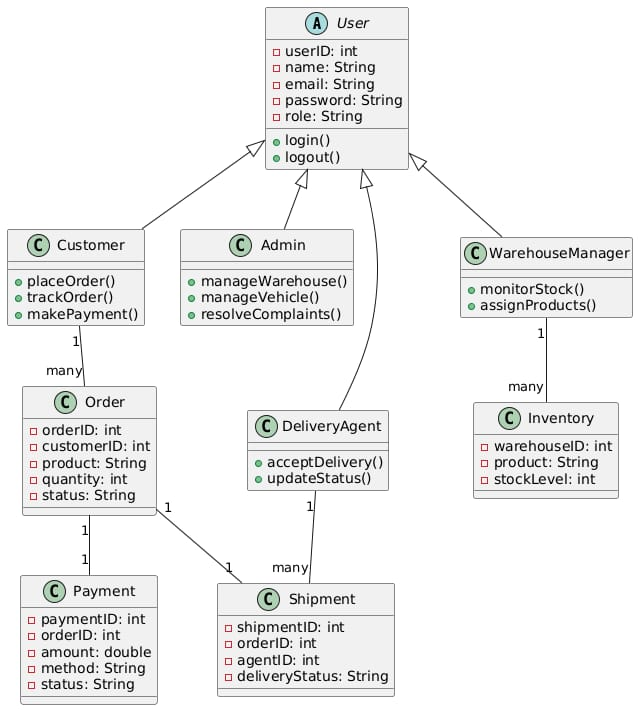
\includegraphics[width=0.8\textwidth]{classdiagram.jpg} 
    \caption{Class Diagram}
    \label{fig:classdiagram}
\end{figure}

\section{Database Design}
The database is designed to store information about users, products, warehouses, retailers, vehicles, orders, payments, and tracking. It supports all system functionalities and ensures relational integrity.

\subsection{User Table}
\begin{longtable}{|l|l|l|}
\hline
\textbf{Column} & \textbf{Type} & \textbf{Notes} \\
\hline
user\_id & INTEGER PK & Auto-increment primary key \\
name & TEXT & Full name \\
email & TEXT UNIQUE & Login email \\
password & TEXT & Hashed password \\
role & TEXT & Enum: Customer, Admin, Agent, Manager \\
contact\_number & TEXT & Optional \\
address & TEXT & Optional \\
\hline
\end{longtable}

\subsection{Product Table}
\begin{longtable}{|l|l|l|}
\hline
\textbf{Column} & \textbf{Type} & \textbf{Notes} \\
\hline
product\_id & INTEGER PK & Auto-increment \\
name & TEXT & Product name \\
description & TEXT & Optional \\
price & REAL & Product price \\
quantity & INTEGER & Current stock \\
warehouse\_id & INTEGER FK & References Warehouse table \\
retailer\_id & INTEGER FK & References Retailer table \\
\hline
\end{longtable}

\subsection{Retailer Table}
\begin{longtable}{|l|l|l|}
\hline
\textbf{Column} & \textbf{Type} & \textbf{Notes} \\
\hline
retailer\_id & INTEGER PK & Auto-increment \\
name & TEXT & Retailer name \\
address & TEXT & Physical location \\
contact\_number & TEXT & Optional \\
\hline
\end{longtable}

\subsection{Warehouse Table}
\begin{longtable}{|l|l|l|}
\hline
\textbf{Column} & \textbf{Type} & \textbf{Notes} \\
\hline
warehouse\_id & INTEGER PK & Auto-increment \\
name & TEXT & Warehouse name \\
address & TEXT & Physical location \\
capacity & INTEGER & Max storage units \\
manager\_id & INTEGER FK & References User table (Warehouse Manager) \\
\hline
\end{longtable}

\subsection{Vehicle Table}
\begin{longtable}{|l|l|l|}
\hline
\textbf{Column} & \textbf{Type} & \textbf{Notes} \\
\hline
vehicle\_id & INTEGER PK & Auto-increment \\
vehicle\_type & TEXT & Enum: Truck, Van, Bike, etc. \\
license\_plate & TEXT & Unique \\
status & TEXT & Enum: Available, On Delivery, Maintenance \\
driver\_id & INTEGER FK & References User table (Delivery Agent) \\
current\_location & TEXT & Optional coordinates/address \\
\hline
\end{longtable}

\subsection{Orders Table}
\begin{longtable}{|l|l|l|}
\hline
\textbf{Column} & \textbf{Type} & \textbf{Notes} \\
\hline
order\_id & INTEGER PK & Auto-increment \\
user\_id & INTEGER FK & References User table \\
product\_id & INTEGER FK & References Product table (nullable if shipment only) \\
order\_type & TEXT & Enum: Purchase, Shipment, Transport \\
source\_address & TEXT & Pickup location \\
destination\_address & TEXT & Delivery location \\
status & TEXT & Enum: Pending, In Warehouse, Out for Delivery, Delivered \\
assigned\_agent\_id & INTEGER FK & References User table (Delivery Agent) \\
vehicle\_id & INTEGER FK & References Vehicle table (optional) \\
payment\_status & TEXT & Enum: Pending, Paid, COD \\
created\_at & DATETIME & Timestamp \\
updated\_at & DATETIME & Timestamp \\
\hline
\end{longtable}

\subsection{Payment Table}
\begin{longtable}{|l|l|l|}
\hline
\textbf{Column} & \textbf{Type} & \textbf{Notes} \\
\hline
payment\_id & INTEGER PK & Auto-increment \\
order\_id & INTEGER FK & References Orders table \\
amount & REAL & Payment amount \\
method & TEXT & Enum: Cash, Card, UPI \\
status & TEXT & Enum: Pending, Completed \\
payment\_date & DATETIME & Timestamp \\
\hline
\end{longtable}

\subsection{Tracking Table}
\begin{longtable}{|l|l|l|}
\hline
\textbf{Column} & \textbf{Type} & \textbf{Notes} \\
\hline
tracking\_id & INTEGER PK & Auto-increment \\
order\_id & INTEGER FK & References Orders table \\
agent\_id & INTEGER FK & References User table \\
current\_status & TEXT & Enum: Picked Up, In Warehouse, Out for Delivery, Delivered \\
location & TEXT & Optional coordinates/address \\
updated\_at & DATETIME & Timestamp \\
\hline
\end{longtable}

\subsection{Relationships}
\begin{itemize}[noitemsep]
    \item User (1) → (many) Orders
    \item User (1) → (many) Vehicles (if Delivery Agent drives a vehicle)
    \item Warehouse (1) → (many) Products
    \item Retailer (1) → (many) Products
    \item Orders (1) → (1) Vehicle (optional)
    \item Orders (1) → (1) Tracking
    \item Orders (1) → (1) Payment
\end{itemize}

\section{UI Wireframe}
% UI Images
\begin{figure}[H]
    \centering
    \includegraphics[width=0.7\textwidth]{login.png} 
    \caption{Login Page}
\end{figure}

\begin{figure}[H]
    \centering
    \includegraphics[width=0.7\textwidth]{customer.png} 
    \caption{User Dashboard}
\end{figure}

\begin{figure}[H]
    \centering
    \includegraphics[width=0.7\textwidth]{admin.png} 
    \caption{Admin Dashboard}
\end{figure}

\begin{figure}[H]
    \centering
    \includegraphics[width=0.7\textwidth]{delivery.png} 
    \caption{Delivery Agent Dashboard}
\end{figure}

\begin{figure}[H]
    \centering
    \includegraphics[width=0.7\textwidth]{warehouse.png} 
    \caption{Warehouse Manager Dashboard}
\end{figure}

\section{Technology Stack}
\begin{enumerate}
    \item Frontend: Java Swing
    \item Backend: Java
    \item Database: SQLite with JDBC connectivity
\end{enumerate}

\section{Security and Validation}
\begin{itemize}
    \item \textbf{Authentication:} Role-based login with encrypted credentials.
    \item \textbf{Validation:} Input validation on order placement, payment fields, and delivery updates.
    \item \textbf{Database Integrity:} Constraints to prevent duplicate orders or invalid stock assignments.
    \item \textbf{Secure Payments:} Dummy simulation of transactions with validation checks.
\end{itemize}

\section{Limitations and Assumptions}
\textbf{Limitations:}
\begin{itemize}
    \item Desktop-only application (not web-enabled).
    \item Payment system is simulated, not integrated with real gateways.
    \item Single warehouse simulation for simplicity.
\end{itemize}

\textbf{Assumptions:}
\begin{itemize}
    \item Users provide correct product and delivery information.
    \item Delivery agents and warehouse managers are available during operations.
    \item Database is centralized and accessible by all roles.
\end{itemize}

\section{Appendices}
\subsection{References}
\begin{enumerate}
    \item \href{https://dev.java/}{Java Docs}
    \item \href{https://www.tutorialspoint.com/}{Tutorial Point}
    \item \href{https://www.sqlite.org/docs.html}{SQLite Documentation}
\end{enumerate}

\end{document}
